\label{sec:Methods}

%* coordinates [limit to nonprecessing?]


%As summarized in Section \ref{sec:Executive}, our algorithm provides a parallel scheme to compare generic binary
%waveforms against data, using a low-cost likelihood function and information from the search to reduce computational cost and
%improve performance.  
%
%In this section, we provide the details needed to implement it.  
%
%Rather than dwell on relatively well-understood data handling issues,  we refer the reader to
%Appendix \ref{ap:DiscreteData} for further discussion of operations on discrete time- and frequency- series.

% POINT: Break up the 

A set of data $d(t)$ collected from a gravitational-wave detector is typically decomposed into the inherent noise of the detector and a putative gravitational wave signal:

\begin{equation}
d(t) = h(t) + n(t)\ .
\end{equation}

In the absence of a signal and under the assumption that each detector produces stationary Gaussian noise, the noise $\tilde{n}(f)$ in the $k^{\rm th}$ detector is characterized by its power spectrum $S_k(f)$:
\begin{eqnarray}
\left<\tilde{n}_k(f)^* \tilde{n}_k(f')\right> = \frac{1}{2} S_k(|f|) \delta(f-f')
\end{eqnarray}

In the following discussion, we define a weighted inner-product of two complex Fourier-domain functions $\tilde{a}(f), \tilde{b}(f)$ with a weighting function $1/S(f)$:

\begin{eqnarray} \label{eq:InnerProduct}
\qmstateproduct{a}{b} \equiv 2 \int_{-\infty}^{\infty} df \frac{\tilde{a}^*(f)\tilde{b}(f)}{S(f)}\
\end{eqnarray}

The mode decomposed waveforms $\hat{h}_{lm}$, can be shifted in time in reference 
to a detector relative to the geocentric time via Eq.~(\ref{eq:time_shift}). 
For this reason, the overlap between a single detector data time series  
$d(t)$ and a time-shifted complex function $h(t-t_k)$ is 
%% Plugging Eq.~(\ref{eq:time_shift}) into Eq.~(\ref{eq:InnerProduct}), the overlap between data $d$ and
%% some template $h(t_k)$ with time of arrival $t_k$ is
\begin{equation} \label{eq:IFFT}
\langle h(t_k) | d \rangle = \int_{-\infty}^{\infty} \frac{\tilde{d}(f) \tilde{h}^*(f)}{S_n(f)} e^{2\pi i f t_k} df \ .
\end{equation}
Note that this is simply the Fourier transform of the integrand in Eq.~(\ref{eq:InnerProduct}), 
which means we can compute the overlap for all possible time shifts with a single
Fourier transform.



%\subsection{Preliminaries}
%We begin with the division of the parameter space of compact binary coalescence waveforms. We first define the difference between ``intrinsic'' and ``extrinsic'' parameters. We define $\itrprm$ as the set of intrinsic parameter as those corresponding to the physical configuration of a binary with component masses $m_1$ and $m_2$: $\itrprm=\{\mc,\eta,\Lambda_1,\Lambda_2,\vec{S}_1,\vec{S}_2\}$, where $\mc$ and $\eta$ are the chirp mass ($(m_1m_2)^{3/5}/(m_1+m_2)^{1/5}$) and symmetric mass ratio ($m_1m_2/(m_1+m_2)^2$), $\Lambda_1$ and $\Lambda_2$ are the tidal numbers of each component mass\footnote{Black holes have no tidal number and thus $\Lambda=0$}, and finally $\vec{S}_1$ and $\vec{S}_2$ correspond to the spin vectors of the component compact objects\footnote{$\vec{L}$, the overall angular momentum of the system is important in the case where the spins are not aligned with the orbital angular momentum, thus causing precession of the orbital plane}. We emphasize in this work rapid determination of source masses --- and possibly compact object type --- thus focusing attention exclusively on $\itrprm=\{\mc,\eta\}$. While the impact of spin and tidal parameters on the waveform are important, they are also potentially complicate the computation of the likelihood in the scheme described later. We thus leave the remaining intrinsic parameters to be built upon in future work.
%
%The extrinsic parameters can be interpreted as the effect of the waveform's arrival and response on a given gravitational-wave detector. For a set of gravitational-wave interferometers, a seven-dimensional space of extrinsic parameters is defined as $\etrprm=\{t_r,\alpha,\delta,\iota,D,\psi,\phi\}$, where $t_r$ is a reference time (in this work, the geocentric time of coalescence), $\alpha$ and $\delta$ are the right ascension and declination, $\iota$ is the inclination angle of the binary's angular momentum vector and the line of sight to Earth, $D$ is the luminosity distance to the binary\footnote{For the sources considered in this paper, the redshift correction is assumed to be negligible}, $\psi$ is the azimuthal angle of the wave's plane of disturbance to the plane of the arms of the detector, and $\phi$ is the orbital phase of the binary at coalescence. Several subsets of these parameters have well-known (particularly in the non-spinning case) correlations.

\subsection{Bayesian evidence and posteriors}
%% We reconstruct the parameter

%% \textbf{Concept}* Top-level review: what are we doing (parameter estimation/posterior); establish notation
%% ($\lambda,\theta,L,p,\ldots$)
%% -----

Here we briefly summarize how Bayes' theorem can be used to quantify how likely it is the data 
(denoted by $\{d\}$) contains only Gaussian noise (hypothesis ${\cal H}_0$) 
or whether it consists of Gaussian noise plus a coherent GW signal in each of our instruments
(hypothesis ${\cal H}_1$). Additionally, it can be used to determine the likely parameters of a signal,
if present.

By our assumption that the noise is Gaussian, it follows that the probability of some set of noise
realizations in each of our detectors is given by
\begin{equation}
p(\{d\}|{\cal H}_0) \propto \prod_k \exp - \frac{ \langle d | d \rangle_k}{2}\ .
\end{equation}
So the data in each detector is noise plus a GW signal 
with true parameters $\vec{\mu}_0$, then the likelihood of some parameters values $\vec{\mu}$ is given by
\begin{equation}
p(\{d\}|\vec{\mu},{\cal H}_1) \propto \prod_k \exp - \frac{ \langle d - h(\vec{\mu}) | d - h(\vec{\mu}) \rangle_k }{2}\ .
\end{equation}
In essence, we subtract a waveform with parameters $\vec{\mu}$ from the data 
and compute how consistent the residual is with Gaussian noise.

We compute an odds ratio $Z$ to quantify the likelihood of a signal relative to the null hypothesis:
\begin{equation} \label{eq:def:Z:Modified}
Z(\{d\}|{\cal H}_1) \equiv \frac{p(\{d\}|{\cal H}_1)}{p(\{d\}|{\cal H}_0)} 
  = \int d\vec{\mu}\ p(\vec{\mu}|{\cal H}_1) \Like(\vec{\mu}|\{d\})\ .
\end{equation}
Here $p(\vec{\mu}|{\cal H}_1)$ is the prior probability for the parameters $\vec{\mu}$ and $\Like(\vec{\mu}|\{d\})$
is the \emph{likelihood ratio}:
\begin{equation} \label{eq:likelihood}
\Like(\vec{\mu}|\{d\}) = \prod_k \frac{\exp - \langle d - H(\vec{\mu}) | d - H(\vec{\mu}) \rangle_k / 2}
{\exp - \langle d | d \rangle_k / 2}\ .
\end{equation}

In addition to the odds ratio, we can also compute the posterior probability density 
(which we will abbreviate as simply the posterior)
for one or multiple parameters (marginalized over all other parameters). Let $x$ be one or more parameters in
$\vec{\mu}$ and $y$ be all other parameters, such that $\vec{\mu} = x \cup y$. Then, the posterior for $x$ is
\begin{equation} \label{eq:def:Posterior}
p({\cal H}_1|x) \equiv \frac{p(x|{\cal H}_1)}{Z(\{d\}|{\cal H}_1)} \ \int dy \;  p(y|{\cal H}_1) \Like(x,y)\ .
\end{equation}
%\editremark{[Do we like the $p_{\rm post}$ notation for posterior?]}

\subsection{Efficiently evaluating the likelihood}

We now show how the waveform decomposition derived above can be exploited
to speed up evaluations of the likelihood ratio.
In Eq.~(\ref{eq:decomposed_strain}) note that we have taken the observed strain in a detector $H_k(t)$
and rewritten it as a linear combination of harmonic mode time series $\hat{h}_{lm}(t)$.
The harmonic mode time series depend on the intrinsic parameters, but
the extrinsic parameters (apart from $t_k$) are entirely encoded in the coefficients of the linear combination.
Because computing the likelihood is just an inner product, which is a linear operator, 
we can pull these coefficients outside the inner product integral.
Thus, we need only compute inner products involving the $\hat{h}_{lm}$ and data $\{d\}$. 
If we store these, we can compute the likelihood for any extrinsic parameters by simply
recomputing the coefficients and reconstructing the linear combination.

To that end, we define the following quantities:
\begin{subequations}
%\label{eq:ComputeRhoViaInnerProductMatrix}
\label{eq:QUV}
\begin{align}
Q_{k,lm}(\itrprm,t_k) &\equiv \qmstateproduct{h_{lm}(\itrprm,t_k)}{d}_k \nonumber\\
&= 2 \int_{-\infty}^{\infty} \frac{df}{S_k(|f|)} e^{2\pi i f t_k} \tilde{h}_{lm}^*(\itrprm;f) \tilde{d}(f)\ , \\
{ U_{k,lm,l'm'}(\lambda)}& = \qmstateproduct{h_{lm}}{h_{l'm'}}_k\ , \\
V_{k,lm,l'm'}(\lambda)& = \qmstateproduct{h_{lm}^*}{h_{l'm'}}_k  \ .
\end{align}
\end{subequations}
Note that each $Q_{k,lm}(\itrprm,t_k)$ is computed for all $t_k$ with a single inverse Fourier transform, 
as in Eq.~(\ref{eq:IFFT}). Because GW detectors can localize a signal to a short time window 
on the order of milliseconds, The $Q_{k,lm}(\itrprm,t_k)$ will be sharply peaked as functions of $t_k$ 
and we need only retain the values for a narrow range of $t_k$. To allow for detector arrival times that differ
from the geocenter time, the range of $t_k$ for which we must store the $Q_{k,lm}$ is set by the light travel
time across Earth ($2R_{\oplus}/c\simeq 42 \unit{ms}$).   In this work we store the $Q_{k,lm}$ for a $300$ ms range of
$t_k$.  
Because time-shifting translates all $h_{lm}$ modes together, 
the $U_{k,lm,l'm'}(\lambda)$ and $V_{k,lm,l'm'}(\lambda)$ are independent of $t_k$
and are computed once by a straightforward use of Eq.~(\ref{eq:InnerProduct}).


By plugging Eq.~(\ref{eq:decomposed_strain}) into Eq.~(\ref{eq:likelihood}), taking a log and collecting terms, we obtain
\begin{widetext}
\begin{align}
\ln \Like(\itrprm; \etrprm) 
&= (D_{\rm ref}/D) \text{Re} \sum_k \sum_{lm}(F_k \Y{-2}_{lm})^* Q_{k,lm}(\itrprm,t_k)\nonumber \\
&   -\frac{(D_{\rm ref}/D)^2}{4}\sum_k
\left[
{
|F_k|^2 [\Y{-2}_{lm}]^*\Y{-2}_{l'm'} U_{k,lm,lm'}(\itrprm)
}
% \right. \nonumber \\ & \left.
 {
+  \text{Re} \left( F_k^2 \Y{-2}_{lm} \Y{-2}_{l'm'} V_{k,lm,l'm'} \right)
}
\right]
\label{eq:def:lnL:Decomposed}
\end{align}
\end{widetext}
Importantly, the intrinsic parameters $\itrprm$ enter only through the $Q_{k,lm}$, $U_{k,lm,l'm'}$ and $V_{k,lm,l'm'}$.
These are the dominant cost, as the require computing the orbital dynamics, the $h_{lm}$, inner product integrals
and inverse Fourier transforms. By contrast, the extrinsic parameters enter the $F_k$ and $\Y{-2}_{lm}$,
which are much simpler closed expressions.

Therefore, if we fix a point in the intrinsic parameter space we can compute the
$Q_{k,lm}(\itrprm,t_k)$, $U_{k,lm,l'm'}(\itrprm)$ and $V_{k,lm,l'm'}(\itrprm)$ only once,
vary the extrinsic parameters and compute the likelihood for only the cost of the $F_k$ and $\Y{-2}_{lm}$.
This allows us to efficiently integrate over the extrinsic parameters and obtain a marginalized posterior 
for the intrinsic parameters $p_{\rm post}(\itrprm)$ as in Eq.~(\ref{eq:def:Posterior}).
If we do this for a collection of points in the intrinsic parameter space, we can integrate over $\itrprm$ as
well and obtain the odds ratio $Z$ as in Eq.~(\ref{eq:def:Z:Modified}).
Note that the computation for each point in the intrinsic space is completely independent of the others.
This makes the algorithm embarrassingly parallel and given enough CPU cores the entire analysis can be
run in the time it takes to integrate over the extrinsic parameters (modulo some brief startup and post-processing steps).

The remainder of this section provides more details on the various steps of our algorithm.

%\subsection{Efficiently evaluating the likelihood}

% POINT: Strain formula
%The complex gravitational wave strain $h=h_+-ih_\times $ at any sufficiently distant point ($t,\vec{x}$) from a nonprecessing
 %binary can be efficiently represented using spin-weighted spherical harmonics $h_{lm}$ as
%\begin{align}
%\label{eq:h:Expansion}
%h(t-\vec{x}\cdot \hat{k}) = \sum_{lm} e^{-2i\psi} h_{lm}(t-\vec{x}\cdot \hat{k})  \Y{-2}_{lm}(\iota,-\phi_c)  \frac{d_{\rm ref}}{d}
%\end{align}
%where $d_{\rm ref}$ is some reference distance at which the $h_{lm}$ are evaluated.  
%In this expression, the vector $\hat{k}$ is the propagation direction ($\hat{k}=-\hat{n}$); the angles $(\iota,\psi)$ are the polar angles of the (fixed) orbital angular momentum direction
%relative to the propagation direction $\hat{k}$; $d$ is the distance to the source; and $\phi_c$ is the coalescence
%(orbital) phase. 
%Expressions for $h_{lm}$ are available in the literature 
%\cite{gwastro-pn-MultipoleMomentsNonspinning, gw-astro-mergers-approximations-SpinningPNHigherHarmonics}.  While many
%phenomenological approximations do not explicitly provide a harmonic representation, the leading order term ($h_{22}$) can be
%easily  identified from published literature by comparing those expressions to the above, evaluated at $\iota=\psi=\phi_c=0$.
  
%
%In terms of this complex strain, the response $H_k$ of the $k$th   gravitational wave detector to low-frequency
%radiation \cite{gwastro-GroundBasedResponse-Whelan2008} can
%be described by a linear combination of $h(t)$ and $h^*(t)$, weighted by time-sky-location-dependent coefficients $F_{+,\times}(t,\hat{n})$:
%\begin{align}
%H_k(t) &=F_{+,k}(t,-\hat{k}) h_+(t-\vec{x}_k(t)\cdot \hat{k}) \nonumber \\
% & + F_{\times,k}(t,-\hat{k}) h_\times(t-\vec{x}_k(t)\cdot \hat{k}) \nonumber \\
% &=  \frac{F_k(-\hat{k}) h(t-\vec{x}_k(t)\cdot \hat{k}) }{2} + \frac{F_k^*(-\hat{k})h^*(t-\vec{x}_k(t)\cdot \hat{k})}{2}
%\label{eq:Hh}
%\end{align}
%where in the second expression we adopt a complex antenna pattern $F_k=F_{+,k}+i F_{\times,k}$.  
%
%For simplicity, in this work we will treat the position $\vec{x}_k$ and antenna pattern $F_k$ of each instrument as
%constants.\footnote{The quality of this approximation is in direct proportion to the ratio $|\Delta x|/\lambda$ where
 % $\Delta x$ is the change in detector position over the waveform's duration and $\lambda$ is the longest significant
 % wavelength.   As either this ratio is a small quantity or the detectors are nearly insensitive to $\lambda$,
  %rotation often need not be included.  Moreover, when radiation \emph{does} need to be included, we anticipate a straightforward perturbative and stationary phase
  %approximation can augment the simple procedure described above, allowing the likelihood to be well approximated with
  %a factor few additional filters and scalars.
%}


%Substituting this expansion for $h$ [Eq. (\ref{eq:h:Expansion})] and the individual-detector response
%[Eq. (\ref{eq:Hh})] into the
%likelihood [Eq. (\ref{eq:def:LikelihoodRatio})], we find the likelihood can be expressed as
%\begin{widetext}
%\begin{align}
%\ln \Like(\lambda; \theta) 
%&= (d_{\rm ref}/d) \text{Re} \sum_k \sum_{lm}(F_k(-\hat{k}) e^{-2\psi} \Y{-2}_{lm}(\hat{n}))^* Q_{k,lm}(t-\hat{k}\cdot
%x_k)
%\nonumber \\
%&   -\frac{(d_{\rm ref}/d)^2}{2}\sum_k
%\left[
%{
 %\frac{1}{2}|F_k(-\hat{k})|^2 U_{k,lm,lm'}(\lambda)[\Y{-2}_{lm}(\hat{n})]^*\Y{-2}_{l'm'}(\hat{n})
%}
% \right. \nonumber \\ & \left.
 %{
%+
 %\frac{1}{2} \text{Re} V_{k,lm,l'm'} e^{-4i\psi}F_k^2 \Y{-2}_{lm}(\hat{n})\Y{-2}_{l'm'}(\hat{n})
%}
%\right]
%\label{eq:def:lnL:Decomposed}
%\end{align}
%\end{widetext}
%In this expression, we use $\hat{n}$ as shorthand for $(\iota,-\phi_c)$; define the constant, detector-dependent
%matrices $U,V$ by 
%\begin{subequations}
%\label{eq:ComputeRhoViaInnerProductMatrix}
%\begin{align}
%{ U_{k,lm,l'm'}(\lambda)}& = \qmstateproduct{h_{lm}}{h_{l'm'}}_k \\
%V_{k,lm,l'm'}(\lambda)& = \qmstateproduct{h_{lm}^*}{h_{l'm'}}_k  \;
%\end{align}
%\end{subequations}
%and define the \emph{filtered data series} $Q_{k,lm}(t)$ via 
%\begin{align}
%Q_{k,lm}(\tau) &\equiv \qmstateproduct{{\cal T}_{\tau} h_{lm}}{\hat{H}_k}_k \\
%&= 2 \int_{-\infty}^{\infty} \frac{df}{S_k(|f|)} e^{+2\pi i f \tau} \tilde{h}_{lm}(f)^* \tilde{\hat{H}}_k(f) \\
%\end{align}
%i.e., as the inner product of the time shifted $h_{lm}$ harmonic [$h_{lm}(t+\tau)\equiv [{\cal T}_\tau h_{lm}](t)$] with the data in the $k$th instrument.


% POINT: This is precomputable
%Critically, all intrinsic-parameter dependent terms in   Eq. (\ref{eq:def:lnL:Decomposed}) can be evaluated once for
%each $\lambda$.  Having calculated these constants ($U_{k,lm,l'm'},V_{k,lm,l'm'}$) and time series ($Q_{k,lm}(\tau)$),
%the likelihood can be efficiently evaluated for any choice of extrinsic parameters $\theta$.
%

% POINT: Computational requirements
%This procedure offers striking reductions in the total number of floating point operations needed to evaluate the
%likelihood.
%Given how precisely gravitational wave searches time-localize candidate events, only a \emph{short} stretch of data
%surrounding a candidate gravitational wave event will ever be examined in  detail.  Hence, rather than evaluate $\Like$ by operating on long-duration, densely sampled
%time- or frequency- series, our expression need only act on constants and a few short arrays.  After minimal preprocessing, the total number of
%floating point evaluations needed for any \emph{subsequent} likelihood evaluation at those same parameters $\lambda$ is
%dramatically reduced.  

%
%Since our method employs no assumptions about the structure of $h_{lm}$, this technique for organizing the likelihood
%calculation can be applied to any existing waveform model, including the effective-one-body approximants
%\cite{gw-astro-EOBspin-Tarrachini2012,gw-astro-EOBNR-Calibrated-2009}.  
%Unlike reduced-order or interpolation-based methods, no further coding, tuning, or calibration is required.  
%Our method requires no  additional model- or detector-dependent development  to achieve this performance improvement.  


\subsection{Placement over intrinsic parameters}
\label{sec:itr_placement}

\begin{figure}
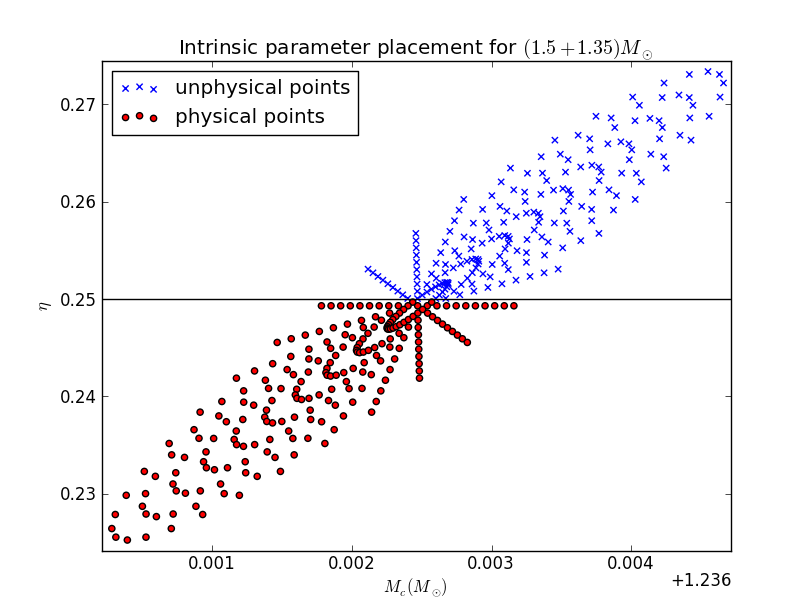
\includegraphics[width=\columnwidth]{../Figures/linear_ellipse_placement.png}
\caption{\label{fig:linear_ellipse} \textbf{Intrinsic parameter placement:} We use an effective Fisher matrix to compute
an approximate ellipsoidal region of overlap $\geq 90\%$ with the masses reported by a detection pipeline.
We then fill this ellipsoid with discrete points and cut any with unphysical values of symmetric mass ratio $\eta$.
At each physical grid point, we marginalize the likelihood over all extrinsic parameters as described in
Sec.~\ref{subsec:extrinsic}.}
\end{figure}

In the current work, we restrict ourselves to considering non-spinning binaries in which we also neglect tidal
effects. Therefore, we need only two mass parameters to describe the intrinsic parameter space, for which we use
the symmetric mass ratio $\eta = m_1 m_2 / M^2$ 
and the chirp mass ${\cal M}_c = M \eta^{3/5}$ (where $M = m_1+m_2$ is the total mass).
Since detection searches will report masses for the candidate event, we use these
to guide which region of the intrinsic parameter space to explore.

Let $\left( {\cal M}^*,\eta^* \right)$ be the masses reported by a detection pipeline. We then perform an effective 
Fisher matrix calculation as described in~\cite{gwastro-mergers-HeeSuk-FisherMatrixWithAmplitudeCorrections,
gwastro-mergers-HeeSuk-CompareToPE-Aligned}
centered about this point.
This involves evaluating the overlap between our waveform with masses $\left( {\cal M}^*,\eta^* \right)$
and $\sim$ tens of nearby waveforms with different intrinsic parameters (while extrinsic parameters are held constant).
The measured overlap values are then fit with a multi-dimensional quadratic. 
The coefficients of this quadratic fit are called the effective Fisher matrix.
Like the standard Fisher matrix, the effective Fisher matrix serves as a quick, crude estimate of expected parameter
estimation performance and can be used to predict surfaces of constant overlap, which will in general be ellipsoids.
In this work, we use the effective Fisher matrix to approximate the region of intrinsic parameter space
which will have overlap $\geq 90\%$ with the masses $\left( {\cal M}^*,\eta^* \right)$.

Once we have defined this $90\%$ overlap ellipsoid, we must fill it with a set of discrete points 
at which we will compute the likelihood. First, we specify the total number of intrinsic parameter points we wish to
place, here  200 points. Then, these points are arranged within a unit sphere. In this work, we placed
points along 20 radial ``spokes'', with 10 points per spoke. Along each spoke, the points are placed 
uniformly in radial distance. Now, the eigenvalues and eigenvectors of the effective Fisher matrix tell us the lengths
and orientations of the axes of the $90\%$ overlap ellipsoid. We use these to deform and rotate our set
of points in the sphere to a set of points in the $90\%$ overlap ellipsoid.
%% One subtlety is that the only physically-meaningful values of $\eta$ are in the range $(0, 0.25]$, but the effective Fisher
%% approach does not account for this physical cutoff. Therefore, for near equal mass binaries where $\eta^* \simeq 0.25$
%% part of the $90\%$ overlap ellipsoid may have unphysical $\eta$ values. 
Once we have filled our ellipsoid, we remove
any points that have unphysical $\eta$ ($>1/4$).   %To counteract this somewhat, 
We ensure that we always place spokes in our ellipsoid along the direction of constant $\eta$,
so that we always have many points along this boundary of the parameter space.
Fig.~\ref{fig:linear_ellipse} illustrates this placement of intrinsic parameter points.

Note that this intrinsic placement routine could be modified in many different ways. 
%% For example, 
%% we could place points uniformly in volume, rather than uniformly in radius. This would place more points
%% towards the edge of the ellipsoid, while we chose uniform-in-radius to get more points near the center.
%% We could also place points randomly inside the ellipse (using uniform-in-volume, uniform-in-radius, 
%% or any other distribution). We chose the spoked placement so that we can always ensure near-equal mass binaries
%% will have many points near the $\eta = 0.25$ boundary of the parameter space.
%% One might also use larger or smaller ellipsoids, use multiple ellipsoids centered at different points if there are concerns
%% about bias in the masses reported by the detection pipeline, choose points according to a metric, 
%% or consider any number of other refinements. 
We plan to refine the intrinsic parameter placement in future work.





\subsection{Integrating over extrinsic parameters}
\label{subsec:extrinsic}

% POINT: General integral form
Because precomputed quantities allow us to efficiently evaluate the likelihood $\Like(\lambda,\theta)$ as a function of
$\theta$, we first integrate the likelihood $\Like(\lambda,\theta)$ over all extrinsic parameters $\theta$:
\begin{eqnarray}
\LikeRed(\lambda) = \int \Like(\lambda,\theta) p(\theta) d\theta
\end{eqnarray}
where $p(\theta)$ is our prior over the extrinsic  parameters.  We assume the sources analyzed are randomly-oriented and
randomly distributed in the universe out to $D_{\rm max}=300 \unit{Mpc}$.  
%% \begin{eqnarray}
%% p(d)=  3 d^2/d_{\rm max}^3 \quad d_{\rm max} = 300\unit{Mpc} \\
%% \end{eqnarray}
% POINT: Specific separable prior, sampling priors approach
To be concrete, we evaluate the reduced likelihood $\LikeRed$ by integrating over sky position $\Omega_{\rm sky}$ represented
as right ascension $\alpha$ and declination $\delta$; angular momentum orientation, measured by inclination $\iota$ and
polarization angle $\psi$;  and coalescence phase $\phi_{\rm c}$, using the separable prior implicitly provided by the
following integral:
\begin{eqnarray}
\LikeRed(\lambda) = \int \frac{dt}{T_{\rm window}} \frac{d^2 dd d\Omega_{sky} }{V_{\rm max}} \frac{d \cos \iota d\phi_c}{4\pi} \frac{d\psi}{\pi} \Like(\lambda,\theta)
\end{eqnarray}
%
In this expression and our calculations, we adopt a maximum distance $d_{\rm max}$ (here $300 \unit{Mpc}$) and a time window
$ T_{\rm window}$  (here, $300\unit{ms}$)  surrounding the event.  

% POINT: MC
With the exception of time (described below), we evaluate these integrals and reconstruct the posterior distribution using Monte Carlo integration
\cite{book-mm-NumericalRecipies,peter1978new}.   To establish notation used below, we briefly review the general principles  underlying Monte Carlo
integration.  If $p_s$ is a distribution which is never zero when $p>0$, then 
\begin{eqnarray}
\LikeRed(\lambda) = \int \frac{\Like(\lambda,\theta) p(\theta)}{p_s(\theta)} [p_s(\theta) d\theta]
\end{eqnarray}
% POINT: Integral value and its error
% 
If we draw $N$ random samples $\theta_q$ from $p_s$, we can estimate the value $\hat{{\cal L}}_{\rm red}$ of $\LikeRed$ and its error using the
expectation value and central limit theorems for independent, identically-distributed random variables:
\begin{eqnarray}
w_q \equiv \frac{\Like(\lambda,\theta_q) p(\theta_q)}{p_s(\theta_q)} \\
\hat{{\cal L}}_{\rm red}(\lambda) \equiv \frac{1}{N} \sum_q w_q = \left<w\right> \\
\sigma_{\LikeRed}^2 = \left<w^2\right> - \left<w\right>^2
\end{eqnarray}
% POINT: Recombinable
Being a pure Monte Carlo integral, we can  combine the results of multiple independent draws of $N$ events, even if these
evaluations adopted different sampling prior.  As a result, this approach is highly parallelizable.  
% Combining results from multiple runs: because pure Monte Carlo, can combine results after multiple runs, using formula


% POINT: PDF reconstruction
The weighted samples also provide an estimate of the marginalized one-dimensional cumulative distributions $P(<x)$ at
fixed $\lambda$, where $x$ is one of the extrinsic variables in $\theta$:
\begin{eqnarray}
\hat{P}(<x) \equiv \frac{1}{\sum_q w_q} \sum_q w_q \theta(x-x_q)
\end{eqnarray}
[This formula follows by performing Monte Carlo integration on the parameter volume $<x$, keeping track of overall
  normalization.]  
In the limit of many samples, this discontinuous estimate should converge to a smooth, marginalized posterior
  distribution.  
%
For any set of samples and any $x$, the error in $\hat{P}$ follows from the (correlated) statistics of the Monte Carlo
integrals in its numerator and denominator; see the Appendix for a rigorous discussion. 
% POINT: neff
In the typical case that all samples $x_q$ are distinct, the unique sample with the largest weight corresponds to the
largest discontinuity in $\hat{P}$.  The magnitude of this discontinuity, or equivalently its inverse $n_{\rm eff}$,
provides a practical measure of how reliable we expect this one-dimensional posterior to be:
\begin{eqnarray}
n_{\rm eff} \equiv \frac{\sum_q w_q}{\text{max} w_{\rm q}}
\end{eqnarray}
Equivalently, the ``effective number of samples'' $n_{\rm eff}$ measures how many independent samples produce similar
weights near the largest observed weight.  
%
Motivated by the effective number of samples and by analogy to the error in a one-dimensional unweighted cumulative
distribution, we expect the standard deviation in our estimate $\hat{P}$ for $P$ to be comparable to or less than the
standard deviation of an \emph{equally-weighted} set of $n_{\rm eff}$ samples,  derived from the binomial distribution:
\begin{eqnarray}
\label{eq:ErrorEstimateCumulative}
\left<\hat{P}^2\right > - \left<\hat{P} \right>^2 \lesssim \frac{P(1-P)}{n_{\rm eff}}
\end{eqnarray}
We \editremark{will} validate this simple estimate.  


%
Unless otherwise indicated, we draw samples using a separable sampling prior $p_s(\alpha) =
\prod_{\alpha}p_{s,\alpha}(\theta_\alpha)$, with each factor $p_{s,\alpha}$ equal to the corresponding prior in that
dimension. 
%% {color{blue} These aren't exceptions: The sampling prior is separable in all parameters unless using a
%% skymap, and then it's effectively $\alpha,\delta\rightarrow\tau$ where $\tau$ is a time delay... 
For some parameters, we adopt a sampling prior that is different than the physical prior, guided by a priori physical
choices; search input;  or past Monte Carlo experience.  These parameters include 
distance (either uniformly or adaptively sampled) and sky position (either uniformly, adaptively, or via a skymap), as
described below.
%

% POINT: How many runs?
Currently, we perform $n_{\rm trials}$ ($=10$) evaluations at each mass point, terminating when either $N$ iterations
crosses a threshold ($=10^6$) or to some fixed
$n_{\rm eff}$ threshold ($=1000$), whichever comes first.  
%
To allow for intrinsic differences in sampling prior between evaluations, the $n_{\rm trials}$ evaluations at each mass
point are
recombined weighted by their (estimated) error: if $\LikeRed_k$  and $\sigma_{\LikeRed,k}$ are the reported integral
values and error estimates for $k=1\ldots n_{\rm trials}$, then
\begin{eqnarray}
\hat{\LikeRed}(\lambda) = \frac{\sum_k \LikeRed_k/\sigma_{\LikeRed,k}^2}{\sum_k 1/\sigma_{\LikeRed,k}^2}
\end{eqnarray}


% POINT: Storage
To mitigate storage requirements, we discard  low-weight samples before recording results.  Low-weight samples are identified by sorting  $w_1<w_2<\ldots$;
constructing the cumulative $W_=\sum_{q\le k} w_q$; and discarding all samples with $W_k/W_N<10^{-4}$.  

\subsubsection{Adaptive Monte Carlo integration}

To better concentrate our samples in regions of high significance, we implemented a simple adaptive Monte Carlo procedure, adjusting
the sampling prior  based on measured weights $w_k$.   The adaptive sampler was used only for selected parameters (i.e.,
distance and sky location), not ubiquitously.   In the long term, we expect to apply more sophisticated adaptive
algorithms, as described in the literature \cite{book-mm-NumericalRecipies,peter1978new}.  For reference, we describe
the specific adaptive algorithm implemented used in this work.


% POINT: Adaptive procedure
Every $n_{\rm chunk}$ samples, we reconstruct the one-dimensional sampling priors in each adapting dimension, using
the last $n_{\rm chunk}\times n_{\rm h}$ samples.    In each dimension ($x$), we subdivide the full range
into $n_{\rm bins}$ equal-length bins $X_\alpha$, then evaluate a tempered, weighted histogram
\begin{eqnarray}
W_\alpha = \frac{\sum_{q} w_q^\beta \Theta_{X_\alpha}(x_q)}{\sum_q w_q^\beta}
\end{eqnarray}
where $\Theta_Y(x)=1$ if  $x$ is in Y and zero otherwise,  and where $\beta$ is a  parameter to moderate the dynamic
range of $w$, described below.  
%
We then \emph{smooth} the array $W$, convolving it with a uniform distribution $n_{\rm smooth}$ bins across.
%
We generated an estimated discrete sampling prior by average the smoothed array $W$ with a uniform distribution with weight $s$:
\begin{eqnarray}
\hat{W}_\alpha = s W + (1-s)/n_{\rm bins}
\end{eqnarray}
% POINT: Discrete to continuous
Finally, we transformed from this discrete, bin-by-bin representation to a continuous integral by (a) constructing
a one-dimensional sampling prior $p_{s,x}(x)$  by interpolating $W^*/\Delta x$ between bin centers, then (b) constructing the
one-dimensional inverse $P_{s,x}(<x)^{-1}$ by integrating $P_{s,x}'(x)=p_{s,x}(x)$.  
%
The latter process ensures that the samplining prior and inverse CDF used to generate random samples are
self-consistent.   
%


% POINT: Specific choices used here
As configured for this paper, we used $n_{\rm bins}=100, n_{\rm hist}=50,n_{\rm smooth}=10,s=0.1$.  We chose the
tempering exponent using the network SNR $\rho$ reported by the search:
\begin{eqnarray}
\beta = \text{min} \left[ 0.8, 4 \frac{\ln (10 n_{\rm chunk})}{\rho^2} \right]
\end{eqnarray}
This choice attempts to mitigate the large dynamic range of $L$ to a scale comparable to the number of samples used in
each histogram.  
%\editremark{We should have changed 10 to nhist...}


%% ---- \editremark{Continue here}

%% * General concept

%% * Specific dimensions adapted

%% * tunings adopted: 100 bins, floor, tempering, history

%% * discard values after burn-in? Not yet....




\subsubsection{Using search results to target specific areas of the sky}

%
Before we begin, gravitational wave search pipelines have usually already identified candidate event times in two or
more interferometers' data, typically to much less than the light crossing time of the earth.  Triangulation limits the
set of candidate sky locations consistent with these results.  Rather than waste time sampling irrelevant sky positions,
we can use search input to immediately target our Monte Carlo at a region of high support.


As a concrete example, the \BS{} pipeline \cite{gw-astro-Bayestar} rapidly processes the results of a gravitational-wave search to identify candidate sky locations consistent with a gravitational wave event with minimal assumptions about the waveform parameters.
%
This code produces a posterior distribution $p_{BS}(\alpha,\delta)$ for the GW signal sky location in a discretized, interlocking, equal-area
grid of pixels corresponding to sky regions, with probabilities for each pixel (a healpix skymap). The refinement of the
grid is variable and scales with the resolution required to resolve the features of the posterior in $\alpha$ and
$\delta$.  
%
%
Using a  distribution, we can construct a sampling prior  $p_s(\alpha,\delta)$.
%
However,  the typical sky resolutions provided by \BS{} are significantly finer than the resolving power of current
gravitational-wave detector networks;   moreover, we are free to adopt higher resolutions as needed.  Hence,  for
simplicity we adopt a purely discrete sky, instead of sampling continuously: the samples are selected from the set of sky
region centers as calculated by the healpix library. These regions are sampled appropriately by their weight in the
posterior.   This method can in principle break down when the true posterior is both large and rapidly changing across
sky pixels.  We will demonstrate efficacy and limitations of a discrete sky by example, below.
%  One possible disadvantage to this is for very sharp features in the posterior, it is possible that this method will fail to find the exact peak of the likelihood function in the sky coordinates. {\color{blue} Can we or should we quantify this?} 

\ForInternalReference{
{\color{blue} The remainder of this explanation is technical and may not be appropriate for the paper. It is here for posterity.} Specifically, the \BS{} pipeline provides a set of $N$ pixels represented as a normalized array of probability mass $s_k$, each index $k$ associated with a pixel centered on $(\alpha_k,\delta_k)$.
%
% Healpy review: http://planck.oat.ts.astro.it/planck/software_and_manuals/Healpix_1.22/Healpix_intro.pdf
%   npix = 12*nside^2 = 49152     %% 4 Pi/(49152)/(Degree)^2 // N
%   nside = 64 (for us)
To generate sky position samples, we generate instead a set of indices corresponding with each index having a multiplicity of $M_k=\frac{s_k}{s_{\text{min}}}\simeq p_s(\alpha_k, \delta_k)$. This represents the probability mass of the region up to an overall quantization error relative to the smallest $s_k$ chosen ($s_{\text{min}}$). The minimum pixel probability is chosen small enough to well represent the quantized probability distribution. {\color{blue} ...and we have a plot of this if necessary}. Finally, a random element of the set is selected and the index chosen is converted back to its sky coordinates $(\alpha_k,\delta_k)$. 
% The point is to avoid rejection sampling which is slow
}

%% POINT: Very high SNR: finer skymaps are available, and we can use

\subsubsection{Time marginalization}
\label{sec:time_marg}

Having already computed all ingredients needed (i.e., $Q_{k,lm}(t)$), we can evaluate the likelihood versus time $\Like(t)$ cheaply, by array
addition operations.  Hence, rather than performing Monte Carlo integration, we can likewise
efficiently \emph{integrate} over time.  

Specifically,  for every sky location drawn by the adaptive Monte Carlo routine, we compute the
corresponding time shift between geocenter and each detector with Eq.~(\ref{eq:t_k}).
To evaluate the value of $\ln {\cal L}$ for some geocenter time $t_{\rm geo}$,
we simply look up the corresponding value of the $Q_{k,lm}(\itrprm,t_k)$ from our precomputed values and plug them
into Eq.~(\ref{eq:def:lnL:Decomposed}).  
%
The resulting time series can be trivially integrated over  $t_{\rm geo}$ by performing a finite sum; see
Appendix \ref{ap:DiscreteData} for details. 





\subsection{Postprocessing: intrinsic priors, interpolation, and the final results}

% POINT: Interpolating in intrinsic parameters
At this point, we have evaluated $\LikeRed(\lambda)$ over a structured grid of intrinsic parameters $\lambda_\mu$.  
%
By construction,  the values $\LikeRed(\lambda)$ have small statistical errors (e.g., less than $1\%$).   Using standard
interpolation packages, we interpolate $\LikeRed(\lambda)$ throughout the sampled grid.\footnote{For example, for linear
spoked interpolation in two dimensions, we adopt polar coordinates that are compatible with the 2d polar grid.}
%
Combined with the prior $p(\lambda)$ over intrinsic parameters, we evaluate the overall evidence $Z$ and posterior
distribution $p_{\rm post}(\lambda)$ over intrinsic parameters via
\begin{eqnarray}
Z = \int d\lambda p(\lambda) \LikeRed(\lambda) \\
p_{\rm post}(\lambda) = \frac{1}{Z} p(\lambda) \LikeRed(\lambda)
\end{eqnarray}
%

% POINT: What about posteriors in 
Similarly, we can construct a posterior distribution over some \emph{extrinsic} parameter $x$ by averaging the one-dimensional posterior estimates derived at
each mass point, weighting each by the prior $p(\lambda)$:
\begin{eqnarray}
P_{\rm post}(<x) = \frac{\int d\lambda P_\lambda(<x) \LikeRed(\lambda) p(\lambda)}{\int d \lambda p(\lambda) \LikeRed(\lambda)}
\end{eqnarray}
This weighted average requires interpolating both $\LikeRed(\lambda)$ and $P_\lambda(<x)$ over all $\lambda$.  


% POINT
%\editremark{Lazy, current approximation}
To a good approximation, however, the intrinsic and extrinsic parameter distributions often separate after marginalizing
in time.  In other words, after marginalizing in time, the extrinsic parameter distributions are nearly independent of $\lambda$.  
In that case, the level of caution exercised above is unwarranted:  each individual
extrinsic parameter distribution provides a reliable estimate of the posterior.  As a crude approximation to the posterior distribution $p_{\rm post}(\theta)$, we  simply \emph{combine} all
weighted samples $(x_{\mu,q},w_{\mu,q})$ from all mass points $\mu$:
\begin{eqnarray}
\hat{P}(<x) = \frac{\sum_{q\mu} w_{q,\mu}\theta(x-x_{\mu,q})}{\sum_{q\mu} w_{q\mu}}
\end{eqnarray}
[This expression agrees with the general approach, for the specific prior implied by the uniform, spoked grid.]
{\color{blue} Feedback?}


